%(BEGIN_QUESTION)
% Copyright 2015, Tony R. Kuphaldt, released under the Creative Commons Attribution License (v 1.0)
% This means you may do almost anything with this work of mine, so long as you give me proper credit

Beregn strømmen gjennom $R_3$ i denne delen av en krets, samt spenningen mellom punkt A og D. Anta at alle motstandene er 1 k$\Omega$:

$$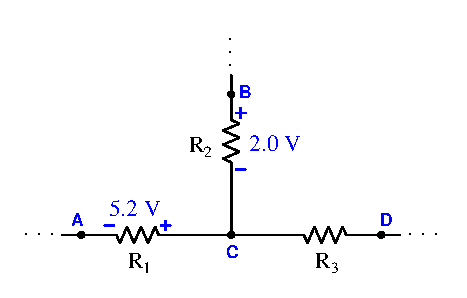
\includegraphics[width=15.5cm]{i00443x01.eps}$$

$I_{R3}$ =

\vskip 10pt

$V_{AD}$ =

\vskip 10pt

\underbar{file i00443}
%(END_QUESTION)





%(BEGIN_ANSWER)

$I_{R3}$ = 3.2 mA

\vskip 10pt

$V_{AD}$ = 8.4 V

%(END_ANSWER)





%(BEGIN_NOTES)

{\bf Dette spørsmålet er ment for eksamen og ikke for arbeidsark!}.

%(END_NOTES)
